\let\negmedspace\undefined
\let\negthickspace\undefined
\documentclass[journal]{IEEEtran}
\usepackage[a5paper, margin=10mm, onecolumn]{geometry}
%\usepackage{lmodern} % Ensure lmodern is loaded for pdflatex
\usepackage{tfrupee} % Include tfrupee package

\setlength{\headheight}{1cm} % Set the height of the header box
\setlength{\headsep}{0mm}     % Set the distance between the header box and the top of the text

\usepackage{gvv-book}
%\usepackage{gvv}
\usepackage{cite}
\usepackage{amsmath,amssymb,amsfonts,amsthm}
\usepackage{algorithmic}
\usepackage{graphicx}
\usepackage{textcomp}
\usepackage{xcolor}
\usepackage{txfonts}
\usepackage{listings}
\usepackage{enumitem}
\usepackage{mathtools}
\usepackage{gensymb}
\usepackage{comment}
\usepackage[breaklinks=true]{hyperref}
\usepackage{tkz-euclide} 
\usepackage{listings}
\usepackage{gvv}                                        
\def\inputGnumericTable{}                                 
\usepackage[latin1]{inputenc}                                
\usepackage{color}                                            
\usepackage{array}                                            
\usepackage{longtable}                                       
\usepackage{calc}                                             
\usepackage{multirow}                                         
\usepackage{hhline}                                           
\usepackage{ifthen}                                           
\usepackage{lscape}
\begin{document}

\bibliographystyle{IEEEtran}

\title{4.2.22}
\author{EE25BTECH11019 - Darji Vivek M.}
{\let\newpage\relax\maketitle}

\renewcommand{\thefigure}{\theenumi}
\renewcommand{\thetable}{\theenumi}
\setlength{\intextsep}{10pt}
\numberwithin{figure}{enumi}
\renewcommand{\thetable}{\theenumi}
\textbf{Question}:\\
Show that the two lines
\[
a_1 x + b_1 y + c_1 = 0,\qquad a_2 x + b_2 y + c_2 = 0
\]
with \(b_1 b_2\neq 0\) are parallel iff \(\dfrac{a_1}{b_1}=\dfrac{a_2}{b_2}\).
\\
\solution

Matrix form:
\begin{align}
\myvec{a_1 & b_1\\ a_2 & b_2}\myvec{x\\y} 
= -\myvec{c_1\\c_2}.
\end{align}

Augmented matrix:
\begin{align}
\augvec{2}{1}{
a_1 & b_1 & -c_1\\
a_2 & b_2 & -c_2
}.
\end{align}

Perform row-reduction:
\begin{align}
R_2 \to R_2 - \frac{a_2}{a_1}R_1
\implies
\augvec{2}{1}{
a_1 & b_1 & -c_1\\
0 & \frac{a_1b_2 - a_2b_1}{a_1} & -c_2 + \frac{a_2c_1}{a_1}
}.
\end{align}

For two lines to be parallel, the coefficient matrix must have rank 1 and the augmented matrix must have rank 2.

Thus,
\begin{align}
a_1b_2 - a_2b_1 = 0.
\end{align}

\(\therefore\) The two lines are parallel if
\begin{align}
\frac{a_1}{b_1} = \frac{a_2}{b_2}, \quad \text{where } b_1b_2 \neq 0.
\end{align}

\begin{figure}[H]
\centering
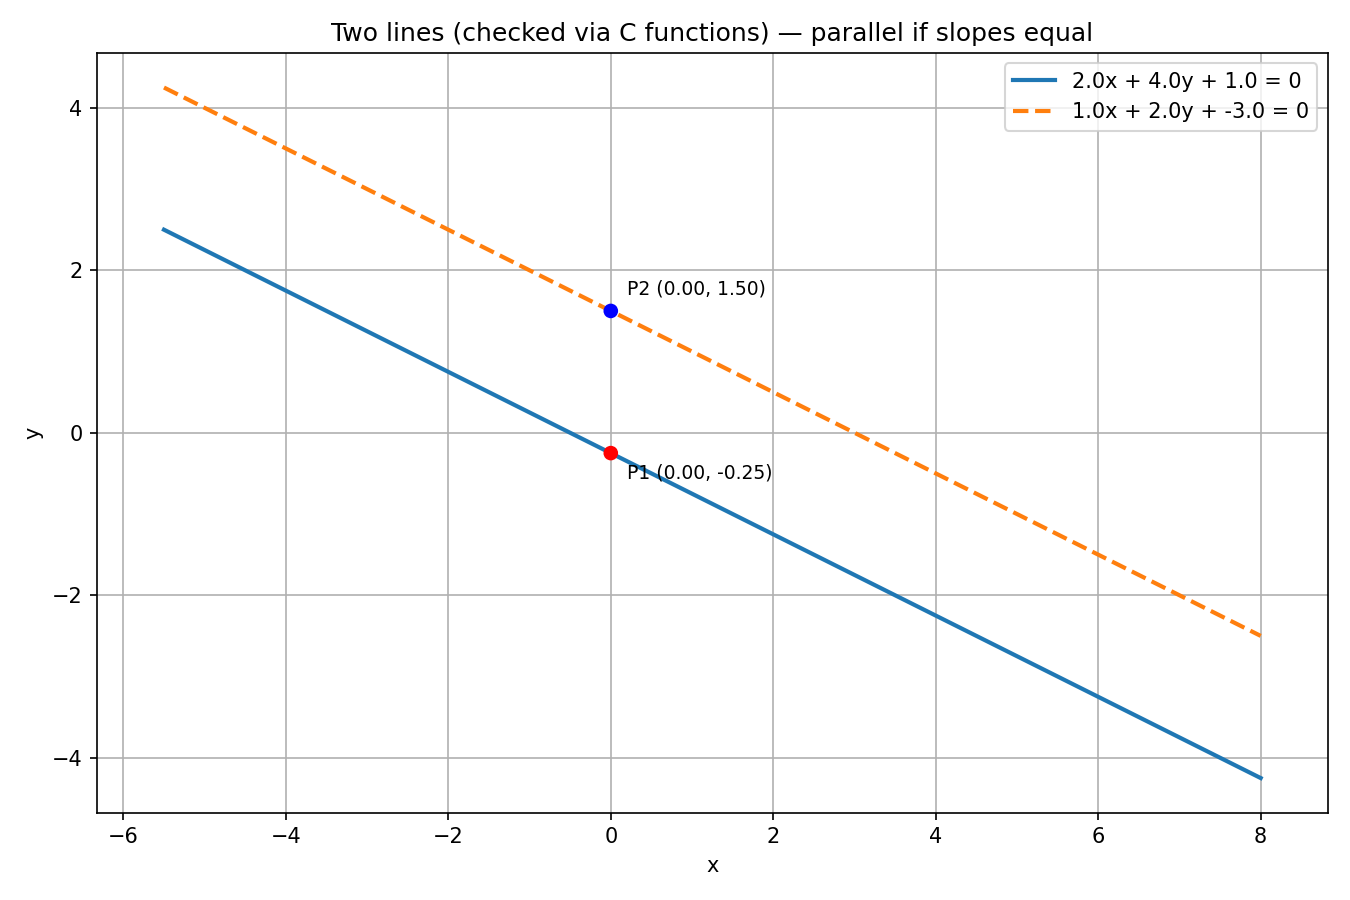
\includegraphics[width=0.75\columnwidth]{figs/6.png}
\caption{\centering plot}
\label{fig:placeholder_125}
\end{figure}
\end{document}
